\subsection{Language coverage}

The first statistics consists of determining how much of the language is covered by the k most used words. The result is shown in figure \ref{coverage_figure}. We could see that, with the same amount of words, we cover less and less of the language from 1840 to 1995.

\begin{figure}[H]
	\centering
    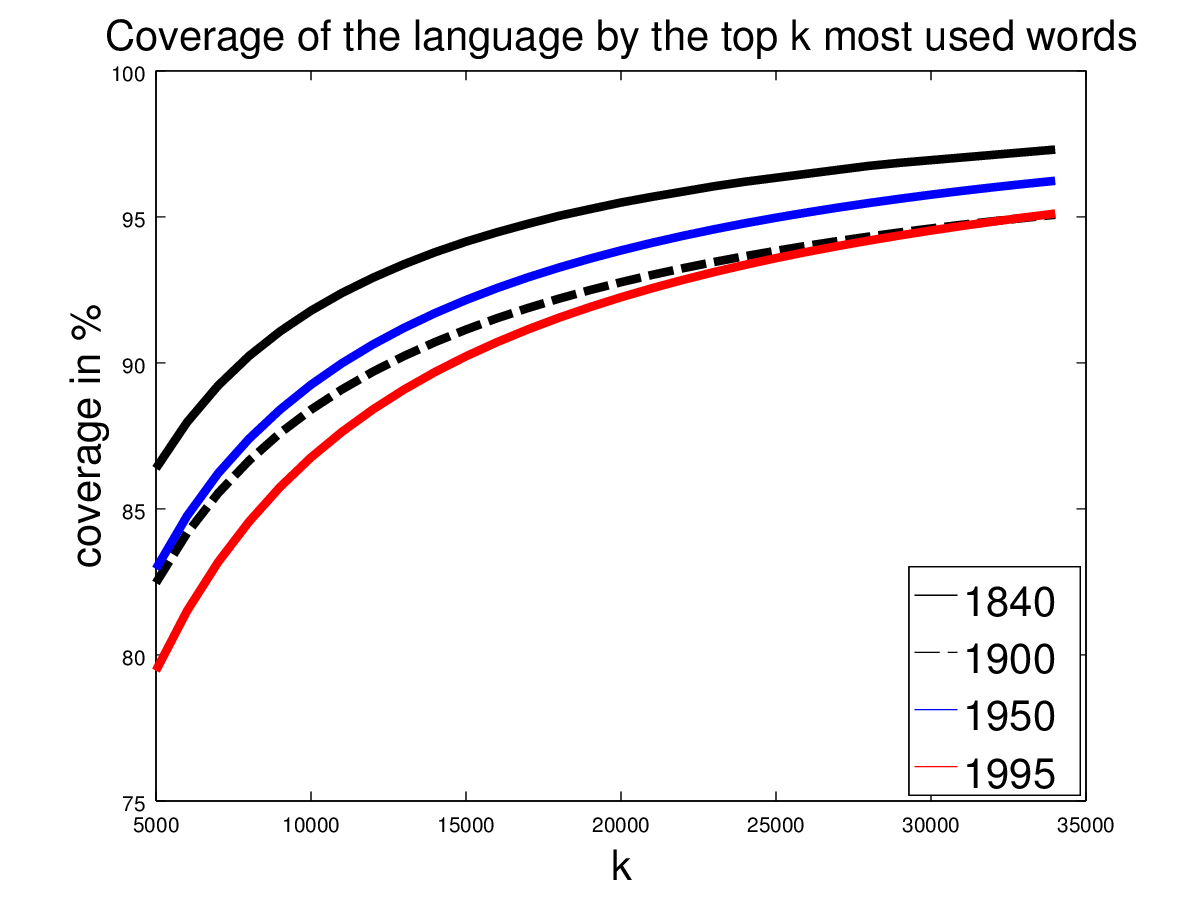
\includegraphics[scale=0.50]{Pictures/statistics/top-k-words-coverage/coverage.png}
    \caption{Percentage of text covered by the top k most used words}
    \label{coverage_figure}
\end{figure}

From those result, we can conclude that the number of new words grows faster with time passing than the number of disappearing words.
%This phenomena could be due to a faster appearance of words than disappearance but could also just show that there is a bigger variation in the vocabulory we use with time.
